% Revised edition: 13 motivation frames inserted before the relevant concepts.
% See insertion_guide.md for original/revised page mapping and teaching prompts.
% COMP 5212 lecture deck: Rademacher Complexity and VC Dimension
% Core organization, definitions, theorems, and proof strategy follow Chapter 3 of:
% M. Mohri, A. Rostamizadeh, and A. Talwalkar,
% Foundations of Machine Learning, 2nd ed., MIT Press, 2018.
% Official author lecture slides were also consulted.
%
% Instructor-added material: pacing, checkpoint questions, geometric redraws,
% toy computations, and numerical examples.
%
% No external images are required. All diagrams are drawn in TikZ.
% The source uses explicit font sizes rather than oversized text commands.

\documentclass[aspectratio=169,10pt]{beamer}

\usepackage[T1]{fontenc}
\usepackage[utf8]{inputenc}
\usepackage{lmodern}
\usepackage{amsmath,amssymb,mathtools}
\usepackage{array,booktabs,multirow}
\usepackage{tikz}
\usetikzlibrary{arrows.meta,positioning,shapes.geometric,calc,fit,backgrounds,decorations.pathreplacing}
\usepackage{hyperref}

% -----------------------------------------------------------------------------
% Visual style: consistent with the earlier COMP 5212 decks
% -----------------------------------------------------------------------------
\definecolor{slideorange}{HTML}{D62B09}
\definecolor{bulletgreen}{HTML}{A8C9A0}
\definecolor{bulletgray}{HTML}{D9E1E8}
\definecolor{deepblue}{HTML}{234A84}
\definecolor{softblue}{HTML}{EAF1FA}
\definecolor{softorange}{HTML}{FBEDE7}
\definecolor{softgreen}{HTML}{EDF5EB}
\definecolor{softgray}{HTML}{F2F3F5}
\definecolor{midgray}{HTML}{666666}
\definecolor{darkgreen}{HTML}{2F7A45}
\definecolor{darkred}{HTML}{A1261A}
\definecolor{pointblue}{HTML}{4E79A7}
\definecolor{pointred}{HTML}{D95F59}
\definecolor{pointgold}{HTML}{D6A84B}

\hypersetup{colorlinks=true,urlcolor=deepblue,linkcolor=deepblue}
\urlstyle{same}

\setbeamertemplate{navigation symbols}{}
\setbeamercolor{background canvas}{bg=white}
\setbeamercolor{normal text}{fg=black,bg=white}
\setbeamercolor{frametitle}{fg=slideorange,bg=white}
\setbeamercolor{page number in head/foot}{fg=black,bg=white}
\setbeamercolor{block body}{bg=softblue,fg=black}
\setbeamercolor{block title}{bg=deepblue,fg=white}
\setbeamercolor{alerted text}{fg=darkred}
\setbeamerfont{frametitle}{series=\bfseries,size*={25pt}{29pt}}
\setbeamerfont{page number in head/foot}{size=\scriptsize}
\setbeamersize{text margin left=0.90cm,text margin right=0.90cm}

\setbeamertemplate{frametitle}{%
  \vspace*{0.12cm}%
  \centering
  {\usebeamerfont{frametitle}\usebeamercolor[fg]{frametitle}\insertframetitle\par}%
  \vspace*{0.10cm}%
}

\setbeamertemplate{footline}{%
  \leavevmode
  \begin{beamercolorbox}[wd=\paperwidth,ht=0.42cm,dp=0.15cm,center]{page number in head/foot}
    \insertframenumber
  \end{beamercolorbox}%
}

\setbeamertemplate{itemize item}{%
  \raisebox{0.15ex}{\tikz\fill[bulletgreen] (0,0) circle (0.082cm);}%
}
\setbeamertemplate{itemize subitem}{%
  \raisebox{0.15ex}{\tikz\fill[bulletgray] (0,0) circle (0.064cm);}%
}

% -----------------------------------------------------------------------------
% Commands and notation
% -----------------------------------------------------------------------------
\DeclareMathOperator*{\argmin}{arg\,min}
\DeclareMathOperator{\sign}{sign}
\newcommand{\X}{\mathcal{X}}
\newcommand{\Y}{\mathcal{Y}}
\newcommand{\Z}{\mathcal{Z}}
\newcommand{\D}{\mathcal{D}}
\newcommand{\Hc}{\mathcal{H}}
\newcommand{\Gc}{\mathcal{G}}
\newcommand{\Fc}{\mathcal{F}}
\newcommand{\R}{R}
\newcommand{\Rhat}{\widehat{R}_S}
\newcommand{\Rad}{\mathfrak{R}}
\newcommand{\RadS}{\widehat{\mathfrak{R}}_S}
\newcommand{\PiH}{\Pi_{\Hc}}
\newcommand{\vcdim}{\operatorname{VCdim}}
\newcommand{\ind}[1]{\mathbf{1}\!\left\{#1\right\}}
\newcommand{\eps}{\varepsilon}
\newcommand{\pmone}{\{-1,+1\}}
\newcommand{\E}{\mathbb{E}}
\newcommand{\Prb}{\mathbb{P}}
\newcommand{\norm}[1]{\left\lVert #1\right\rVert}
\newcommand{\abs}[1]{\left\lvert #1\right\rvert}
\newcommand{\angles}[1]{\left\langle #1\right\rangle}

\newcommand{\SectionSlide}[2]{%
  \begin{frame}
    \centering
    \vfill
    {\color{slideorange}\fontsize{29}{34}\selectfont\bfseries #1\par}
    \vspace{0.38cm}
    {\color{midgray}\fontsize{16}{21}\selectfont #2\par}
    \vfill
  \end{frame}
}

\newcommand{\BreakSlide}[2]{%
  \begin{frame}
    \centering
    \vfill
    {\color{deepblue}\fontsize{28}{33}\selectfont\bfseries #1\par}
    \vspace{0.35cm}
    {\color{midgray}\fontsize{16}{21}\selectfont #2\par}
    \vfill
  \end{frame}
}

\newcommand{\SourceNote}[1]{%
  \vfill
  \begin{flushright}
    {\scriptsize\color{midgray}#1}
  \end{flushright}
}

\newcommand{\KeyBox}[1]{%
  \begin{beamercolorbox}[rounded=true,sep=0.22cm,wd=\linewidth]{block body}
    #1
  \end{beamercolorbox}%
}

\newcommand{\OrangeBox}[1]{%
  \begin{beamercolorbox}[rounded=true,sep=0.22cm,wd=\linewidth]{alertblock body}
    #1
  \end{beamercolorbox}%
}
\setbeamercolor{alertblock body}{bg=softorange,fg=black}

\begin{document}

% ORIGINAL PDF SLIDE 1: Course title
\begin{frame}
	\begin{tikzpicture}[remember picture, overlay]
		\node[anchor=north west, inner sep=10pt] at (current page.north west)
		{
\includegraphics[width=6cm]{assets/logo.png}};
	\end{tikzpicture}
	
	\centering
	\vspace*{1.15cm}
	{\fontsize{28}{32}\selectfont COMP 5212\par}
	\vspace{0.35cm}
	{\fontsize{30}{33}\selectfont Machine Learning\par}
	\vspace{0.75cm}
	{\Large Instructor: Zihan Zhang\par}
	\vspace{0.35cm}
	{\large Lecture 3: Rademacher Complexity and VC Dimension\par}
	\vspace{0.2cm}
	
\end{frame}


% ORIGINAL PDF SLIDE 2: Learning Goals
\begin{frame}[t]{Learning Goals}
  \vspace{0.03cm}
  {\fontsize{13.2}{16.2}\selectfont
  By the end of the lecture, you should be able to:
  \begin{itemize}
    \setlength{\itemsep}{0.18cm}
    \item define empirical and expected Rademacher complexity;
    \item explain the symmetrization argument behind Rademacher bounds;
    \item connect growth functions to Rademacher complexity via Massart's lemma;
    \item compute or bound the VC dimension of common hypothesis classes;
    \item use Sauer's lemma to derive generalization guarantees for VC classes.
  \end{itemize}}
\end{frame}


% ORIGINAL PDF SLIDE 3: Infinite Hypothesis Sets
\begin{frame}[t]{Infinite Hypothesis Sets}
  \vspace{0.04cm}
  \begin{columns}[T,totalwidth=\textwidth]
    \begin{column}{0.52\textwidth}
      \begin{itemize}
        \setlength{\itemsep}{0.13cm}
        \item Linear classifiers contain infinitely many parameter choices $(w,b)$.
        \item Intervals on $\mathbb{R}$ contain infinitely many endpoint pairs.
        \item Neural networks and kernel predictors form even richer classes.
      \end{itemize}
      \vspace{0.08cm}
      The finite-class term
      \[
        \sqrt{\frac{\log\abs{\Hc}}{m}}
      \]
      is meaningless when $\abs{\Hc}=\infty$.
    \end{column}
    \begin{column}{0.46\textwidth}
      \begin{center}
      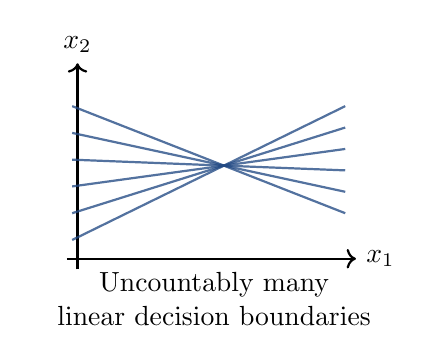
\begin{tikzpicture}[scale=0.68]
        \draw[->,thick] (-0.2,0) -- (5.2,0) node[right] {$x_1$};
        \draw[->,thick] (0,-0.2) -- (0,3.65) node[above] {$x_2$};
        \foreach \b/\s in {0.35/0.50,0.85/0.32,1.35/0.14,1.85/-0.04,2.35/-0.22,2.85/-0.40}{
          \draw[deepblue,opacity=0.78,thick] (-0.1,{\b}) -- (5,{\b+\s*5});
        }
        \node[align=center,text width=4.5cm] at (2.55,-0.75) {Uncountably many\\linear decision boundaries};
      \end{tikzpicture}
      \end{center}
    \end{column}
  \end{columns}
\end{frame}

% ORIGINAL PDF SLIDE 4: Why the Naive Union Bound Fails
\begin{frame}[t]{Why the Naive Union Bound Fails}
  \vspace{0.06cm}
  For a fixed $h$, concentration gives approximately
  \[
    \Prb\!\left(\abs{R(h)-\Rhat(h)}>\eps\right)
    \le 2e^{-2m\eps^2}.
  \]
  For finite $\Hc$, a union bound yields
  \[
    \Prb\!\left(\sup_{h\in\Hc}\abs{R(h)-\Rhat(h)}>\eps\right)
    \le 2\abs{\Hc}\,e^{-2m\eps^2}.
  \]
  \vspace{0.05cm}
  \begin{beamercolorbox}[rounded=true,sep=0.20cm,wd=\linewidth]{alertblock body}
    When $\abs{\Hc}=\infty$, this gives no information. We need to measure only the distinctions the class can make on finite samples.
  \end{beamercolorbox}
\end{frame}

% ORIGINAL PDF SLIDE 5: Three Views of Capacity
\begin{frame}[t]{Three Views of Capacity}
  \vspace{0.10cm}
  \begin{center}
  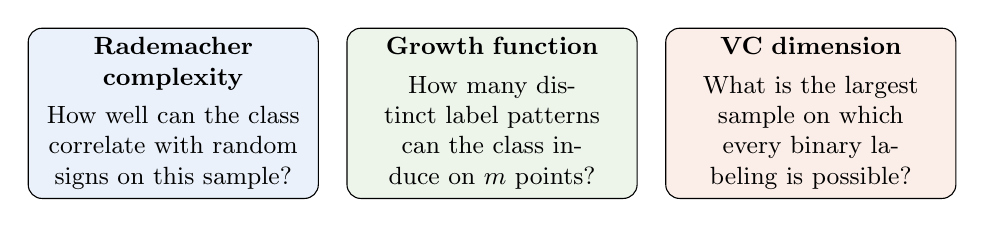
\begin{tikzpicture}[
      card/.style={draw=black,rounded corners=5pt,text width=3.45cm,minimum height=2.15cm,align=center,fill=softgray,font=\small},
      node distance=0.35cm
    ]
    \node[card,fill=softblue] (r) {\textbf{Rademacher complexity}\\[0.10cm]
      How well can the class correlate with random signs on this sample?};
    \node[card,right=of r,fill=softgreen] (g) {\textbf{Growth function}\\[0.10cm]
      How many distinct label patterns can the class induce on $m$ points?};
    \node[card,right=of g,fill=softorange] (v) {\textbf{VC dimension}\\[0.10cm]
      What is the largest sample on which every binary labeling is possible?};
  \end{tikzpicture}
  \end{center}
  \vspace{0.22cm}
  \centering
  \textbf{Analytic} $\longrightarrow$ \textbf{combinatorial} $\longrightarrow$ \textbf{single-number summary}

\end{frame}

% ORIGINAL PDF SLIDE 6: Part I: Rademacher Complexity
\SectionSlide{Part I: Rademacher Complexity}{}



\begin{frame}[t]{Random Signs as a Stress Test}
  \vspace{0.10cm}
  Fix a sample $S=(z_1,\ldots,z_m)$ and draw independent signs
  \[
    \sigma_1,\ldots,\sigma_m\sim\operatorname{Unif}\pmone.
  \]
  For each $g\in\Gc$, measure the correlation
  \[
    \frac{1}{m}\sum_{i=1}^m \sigma_i g(z_i).
  \]
  \vspace{0.08cm}
  \begin{columns}[T,totalwidth=\textwidth]
    \begin{column}{0.49\textwidth}
      \KeyBox{A simple class cannot systematically align with independent random signs.}
    \end{column}
    \begin{column}{0.49\textwidth}
      \OrangeBox{A rich class may select a function after seeing the signs and achieve high correlation.}
    \end{column}
  \end{columns}
\end{frame}

% ORIGINAL PDF SLIDE 8: Empirical Rademacher Complexity
\begin{frame}[t]{Empirical Rademacher Complexity}
  \vspace{0.06cm}
  Let $\Gc$ be a family of real-valued functions on $\Z$ and let
  $S=(z_1,\ldots,z_m)$.
  \vspace{0.06cm}
  \begin{beamercolorbox}[rounded=true,sep=0.23cm,wd=\linewidth]{block body}
    \[
      \boxed{
      \RadS(\Gc)
      =\E_{\sigma}\!\left[
        \sup_{g\in\Gc}\frac{1}{m}\sum_{i=1}^m \sigma_i g(z_i)
      \right]}
    \]
    where the $\sigma_i$ are independent Rademacher variables taking values in $\pmone$.
  \end{beamercolorbox}
  \vspace{0.14cm}
  \begin{itemize}
    \setlength{\itemsep}{0.10cm}
    \item The sample is fixed; the expectation is only over random signs.
    \item The supremum chooses the best-fitting function for each sign vector.
    \item The normalization by $m$ makes the scale comparable across sample sizes.
  \end{itemize}
\end{frame}

% ORIGINAL PDF SLIDE 9: Geometry of the Definition
\begin{frame}[t]{Geometry of the Definition}
  \vspace{0.01cm}
  Associate each function with its evaluation vector
  \[
    v_g(S)=\bigl(g(z_1),\ldots,g(z_m)\bigr)\in\mathbb{R}^m.
  \]
  Then
  \[
    \RadS(\Gc)
    =\frac{1}{m}\E_{\sigma}\left[
      \sup_{v\in A_S}\angles{\sigma,v}
    \right],
    \qquad A_S=\{v_g(S):g\in\Gc\}.
  \]
  \begin{center}
  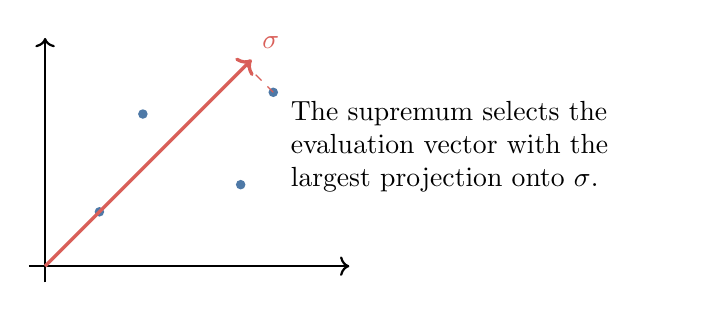
\begin{tikzpicture}[scale=0.69]
    \draw[->,thick] (-0.3,0) -- (5.6,0);
    \draw[->,thick] (0,-0.3) -- (0,4.2);
    \fill[pointblue] (1.0,1.0) circle (2.5pt);
    \fill[pointblue] (1.8,2.8) circle (2.5pt);
    \fill[pointblue] (3.6,1.5) circle (2.5pt);
    \fill[pointblue] (4.2,3.2) circle (2.5pt);
    \draw[->,very thick,pointred] (0,0) -- (3.8,3.8) node[above right] {$\sigma$};
    \draw[dashed,pointred] (4.2,3.2) -- (3.7,3.7);
    \node[align=left,text width=4.8cm] at (8.0,2.2) {The supremum selects the evaluation vector with the largest projection onto $\sigma$.};
  \end{tikzpicture}
  \end{center}
\end{frame}

% ORIGINAL PDF SLIDE 10: Toy Examples: Very Small Classes
\begin{frame}[t]{Toy Examples: Very Small Classes}
  \vspace{0.06cm}
  \begin{columns}[T,totalwidth=\textwidth]
    \begin{column}{0.48\textwidth}
      \textbf{Singleton class $\Gc=\{g_0\}$}
      \[
        \RadS(\Gc)
        =\E_\sigma\frac{1}{m}\sum_i\sigma_i g_0(z_i)=0.
      \]
      There is no choice after seeing the signs.
    \end{column}
    \begin{column}{0.50\textwidth}
      \textbf{Two constant functions $\Gc=\{-1,+1\}$}
      \[
        \RadS(\Gc)
        =\E_\sigma\abs{\frac{1}{m}\sum_i\sigma_i}
        \approx \sqrt{\frac{2}{\pi m}}.
      \]
      The complexity decays like $m^{-1/2}$.
    \end{column}
  \end{columns}
  \vspace{0.20cm}
  \KeyBox{Rademacher complexity measures flexibility of a \emph{class}, not variability of one fixed function.}
\end{frame}

% ORIGINAL PDF SLIDE 11: Toy Example: A Maximally Rich Class
\begin{frame}[t]{Toy Example: A Maximally Rich Class}
  \vspace{0.06cm}
  Suppose that on the fixed sample $S$, the class realizes every sign pattern:
  \[
    \{(g(z_1),\ldots,g(z_m)):g\in\Gc\}=\pmone^m.
  \]
  After observing $\sigma$, choose $g_\sigma$ satisfying $g_\sigma(z_i)=\sigma_i$. Then
  \[
    \sup_{g\in\Gc}\frac{1}{m}\sum_i\sigma_i g(z_i)
    =\frac{1}{m}\sum_i\sigma_i^2=1.
  \]
  Therefore,
  \[
    \boxed{\RadS(\Gc)=1.}
  \]
  \vspace{0.08cm}
  \OrangeBox{A class able to reproduce arbitrary random labels has maximal sample-level complexity.}
\end{frame}


\begin{frame}[t]{Expected Rademacher Complexity}
	\vspace{0.10cm}
	When the sample itself is random, define
	\begin{beamercolorbox}[rounded=true,sep=0.22cm,wd=\linewidth]{block body}
		\[
		\boxed{
			\Rad_m(\Gc)=\E_{S\sim\D^m}\bigl[\RadS(\Gc)\bigr].}
		\]
	\end{beamercolorbox}
	\vspace{0.18cm}
	\begin{itemize}
		\setlength{\itemsep}{0.15cm}
		\item $\RadS(\Gc)$ is \textbf{data-dependent}: it adapts to the observed sample.
		\item $\Rad_m(\Gc)$ is \textbf{distribution-dependent}: it averages over samples from $\D$.
		\item A worst-case upper bound may remove dependence on both $S$ and $\D$, at the cost of looseness.
	\end{itemize}
\end{frame}

\begin{frame}[t]{Repeated and Distinct Inputs}
  \vspace{0.04cm}
  \small

  Let $a$ and $b$ represent two patient profiles. Let $\Hc$ contain all
  four maps $\{a,b\}\to\pmone$.
  Keep this class fixed and compare samples of size two.
  \begin{center}
  \renewcommand{\arraystretch}{1.15}
  \begin{tabular}{lcc}
    \toprule
    & $S_1=(a,a)$ & $S_2=(a,b)$\\
    \midrule
    Available prediction vectors & $(+,+),(-,-)$ & all four sign vectors\\
    Best scores for $++,+-,-+,--$ & $1,0,0,1$ & $1,1,1,1$\\
    Average over random signs & $\widehat{\Rad}_{S_1}=1/2$ & $\widehat{\Rad}_{S_2}=1$\\
    \bottomrule
  \end{tabular}
  \end{center}
  If $a$ and $b$ each have probability $1/2$, an i.i.d. sample repeats a
  point with probability $1/2$. The average over samples is
  \[
    \frac12\cdot\frac12+\frac12\cdot1=\frac34.
  \]
  \KeyBox{The first average fixes the inputs. A second average accounts for
  which inputs the data distribution supplies.}

\end{frame}

% MOTIVATION V02 -- before original PDF page 12: Expected Rademacher Complexity
\begin{frame}[t]{Repeated and Distinct Patients}
  \vspace{0.04cm}\small
  The same risk model can have different flexibility on different samples.
  \begin{center}
  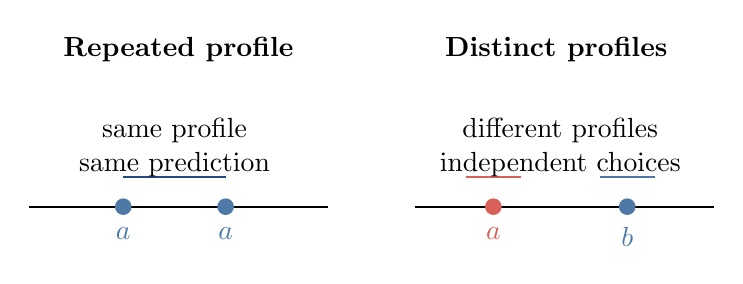
\begin{tikzpicture}[x=1cm,y=1cm]
    \node[font=\bfseries] at (1.9,2.0) {Repeated profile};
    \node[font=\bfseries] at (6.7,2.0) {Distinct profiles};
    \draw[thick] (0,0)--(3.8,0);
    \fill[pointblue] (1.2,0) circle (3pt) node[below=4pt] {$a$};
    \fill[pointblue] (2.5,0) circle (3pt) node[below=4pt] {$a$};
    \draw[deepblue,thick] (1.2,0.38)--(2.5,0.38);
    \node[align=center] at (1.85,0.75) {same profile\\same prediction};
    \draw[thick] (4.9,0)--(8.7,0);
    \fill[pointred] (5.9,0) circle (3pt) node[below=4pt] {$a$};
    \fill[pointblue] (7.6,0) circle (3pt) node[below=4pt] {$b$};
    \draw[pointred,thick] (5.55,0.38)--(6.25,0.38);
    \draw[pointblue,thick] (7.25,0.38)--(7.95,0.38);
    \node[align=center] at (6.75,0.75) {different profiles\\independent choices};
  \end{tikzpicture}
  \end{center}
  \vspace{0.08cm}
  \KeyBox{The first sample forces repeated evaluations to agree. The second
  sample lets the class choose two predictions separately.}
\end{frame}



% ORIGINAL PDF SLIDE 13: Basic Properties
\begin{frame}[t]{Basic Properties}
  \vspace{0.01cm}
  For a fixed sample $S$:
  \begin{align*}
    \Gc\subseteq\Fc
      &\quad\Longrightarrow\quad \RadS(\Gc)\le \RadS(\Fc),\\[0.08cm]
    c\ge 0
      &\quad\Longrightarrow\quad \RadS(c\Gc)=c\RadS(\Gc),\\[0.08cm]
    \Gc+a
      &\quad\Longrightarrow\quad \RadS(\Gc+a)=\RadS(\Gc),\\[0.08cm]
    \RadS(\Gc_1+\Gc_2)
      &\quad\le\quad \RadS(\Gc_1)+\RadS(\Gc_2).
  \end{align*}
  Here $a$ is a fixed function added to every member, and
  $\Gc_1+\Gc_2=\{g_1+g_2:g_j\in\Gc_j\}$.
  \vspace{0.10cm}
  \KeyBox{These rules let us analyze composite function classes from simpler building blocks.}
\end{frame}

% ORIGINAL PDF SLIDE 14: Convexification Does Not Increase Complexity
% MOTIVATION M03 -- before original PDF page 14: Convexification Does Not Increase Complexity
\begin{frame}[t]{Mixing Two Predictors}
  \vspace{0.03cm}
  \small
  Fix one sample $S$ and one sign vector $\sigma$.  Suppose two real-valued
  functions have correlations
  \[
    c_1=\frac1m\sum_i\sigma_i g_1(z_i)=0.2,
    \qquad
    c_2=\frac1m\sum_i\sigma_i g_2(z_i)=0.6.
  \]
  For the mixture $f_\alpha=\alpha g_1+(1-\alpha)g_2$, $0\le\alpha\le1$,
  \[
    \frac1m\sum_i\sigma_i f_\alpha(z_i)
      =\alpha c_1+(1-\alpha)c_2
      =0.6-0.4\alpha\in[0.2,0.6].
  \]
  \vspace{0.02cm}
  \KeyBox{\centering
    The best mixture reaches $0.6$, exactly the better endpoint score.
    We added infinitely many mixtures. Did we gain any ability to fit this
    noise vector? What happens when we average over all sign vectors?
  }

\end{frame}

\begin{frame}[t]{Convexification Does Not Increase Complexity}
  \vspace{0.03cm}
  \small
  Let $\operatorname{conv}(\Gc)$ denote finite convex combinations of functions in $\Gc$. For each sign vector $\sigma$,
  \begin{align*}
    \sup_{f\in\operatorname{conv}(\Gc)}\sum_i\sigma_i f(z_i)
    &=\sup_{\substack{\alpha_j\ge0\\\sum_j\alpha_j=1}}
      \sum_j\alpha_j\sum_i\sigma_i g_j(z_i)\\
    &=\sup_{g\in\Gc}\sum_i\sigma_i g(z_i).
  \end{align*}
  Hence
  \[
    \boxed{\RadS(\operatorname{conv}(\Gc))=\RadS(\Gc).}
  \]
  \vspace{0.08cm}
  \OrangeBox{\footnotesize Convex mixtures can greatly enlarge a class without increasing this complexity; this later helps analyze ensembles.}
\end{frame}


\begin{frame}[t]{From Hypotheses to Loss Functions}
  \vspace{0.06cm}
  Generalization concerns losses, not predictions directly. Given $\Hc$ and loss $\ell$, define
  \[
    \ell\circ\Hc
    =\bigl\{(x,y)\mapsto \ell(h(x),y):h\in\Hc\bigr\}.
  \]
  For binary $h:\X\to\pmone$ with zero-one loss,
  \[
    \Gc=\{(x,y)\mapsto\ind{h(x)\ne y}:h\in\Hc\}.
  \]
  Using $\ind{h(x)\ne y}=\tfrac12(1-yh(x))$ and sign symmetry,
  \[
    \boxed{\Rad_m(\Gc)=\frac12\Rad_m(\Hc).}
  \]
  \SourceNote{This loss-class relation is a central specialization in Chapter 3.}
\end{frame}

% ORIGINAL PDF SLIDE 16: Rademacher Generalization Bound
\begin{frame}[t]{Rademacher Generalization Bound}
  \vspace{0.02cm}
  Let $\Gc$ be a family of functions $g:\Z\to[0,1]$. For any $\delta>0$, with probability at least $1-\delta$ over $S\sim\D^m$, every $g\in\Gc$ satisfies
  \begin{beamercolorbox}[rounded=true,sep=0.18cm,wd=\linewidth]{block body}
    \[
      \E[g(z)]
      \le \frac1m\sum_{i=1}^m g(z_i)
      +2\Rad_m(\Gc)
      +\sqrt{\frac{\log(1/\delta)}{2m}}.
    \]
  \end{beamercolorbox}
  A data-dependent version is
  \begin{beamercolorbox}[rounded=true,sep=0.18cm,wd=\linewidth]{alertblock body}
    \[
      \E[g(z)]
      \le \frac1m\sum_{i=1}^m g(z_i)
      +2\RadS(\Gc)
      +3\sqrt{\frac{\log(2/\delta)}{2m}}.
    \]
  \end{beamercolorbox}
  \SourceNote{Koltchinskii and Panchenko (2002); theorem presentation follows Chapter 3.}
\end{frame}

% ORIGINAL PDF SLIDE 17: How to Read the Bound
\begin{frame}[t]{How to Read the Bound}
  \vspace{0.10cm}
  \[
    \text{population loss}
    \ \le\ \text{training loss}
    +\text{class complexity}
    +\text{confidence penalty}.
  \]
  \vspace{0.10cm}
  \begin{columns}[T,totalwidth=\textwidth]
    \begin{column}{0.32\textwidth}
      \KeyBox{\centering\textbf{Fit}\\$\frac1m\sum_i g(z_i)$}
    \end{column}
    \begin{column}{0.32\textwidth}
      \KeyBox{\centering\textbf{Capacity}\\$2\RadS(\Gc)$}
    \end{column}
    \begin{column}{0.32\textwidth}
      \KeyBox{\centering\textbf{Confidence}\\$O(\sqrt{\log(1/\delta)/m})$}
    \end{column}
  \end{columns}
  \vspace{0.18cm}
  \begin{itemize}
    \setlength{\itemsep}{0.09cm}
    \item The theorem is simultaneous over all $g\in\Gc$.
    \item The complexity term shrinks with $m$ for learnable classes.
    \item The empirical version can be smaller on ``easy'' samples.
  \end{itemize}
\end{frame}



\begin{frame}[t]{Proof Roadmap}
  \vspace{0.05cm}
  Define the worst one-sided gap
  \[
    \Phi(S)=\sup_{g\in\Gc}\left(\E[g]-\widehat{\E}_S[g]\right).
  \]
  The proof has three conceptual moves:
  \vspace{0.04cm}
  \begin{enumerate}
    \setlength{\itemsep}{0.15cm}
    \item \textbf{Concentration:} show $\Phi(S)$ is close to $\E_S\Phi(S)$ by bounded differences.
    \item \textbf{Ghost sample:} replace $\E[g]$ by an independent empirical average.
    \item \textbf{Symmetrization:} random signs convert a two-sample difference into Rademacher complexity.
  \end{enumerate}
  \vspace{0.10cm}
  \centering
  \textbf{Uniform deviation} $\Rightarrow$ \textbf{randomized correlation problem}
\end{frame}

% ORIGINAL PDF SLIDE 19: Step 1: Bounded Differences
\begin{frame}[t]{Step 1: Bounded Differences}
  \vspace{0.01cm}
  Let $S$ and $S'$ differ only in the last point. Since $g\in[0,1]$,
  \begin{align*}
    \Phi(S')-\Phi(S)
    &\le \sup_{g\in\Gc}
      \left(\widehat{\E}_S[g]-\widehat{\E}_{S'}[g]\right)\\
    &=\sup_{g\in\Gc}\frac{g(z_m)-g(z_m')}{m}
    \le \frac1m.
  \end{align*}
  McDiarmid's inequality yields, with probability at least $1-\delta/2$,
  \[
    \Phi(S)
    \le \E_S[\Phi(S)]
    +\sqrt{\frac{\log(2/\delta)}{2m}}.
  \]
  \vspace{0.05cm}
  \KeyBox{The hard part is now to bound the mean $\E_S[\Phi(S)]$.}
\end{frame}

% ORIGINAL PDF SLIDE 20: Step 2: Introduce a Ghost Sample
\begin{frame}[t]{Step 2: Introduce a Ghost Sample}
  \vspace{0.01cm}
  Let $S'=(z_1',\ldots,z_m')\sim\D^m$ be independent of $S$. Then
  \begin{align*}
    \E_S[\Phi(S)]
    &=\E_S\sup_{g\in\Gc}\left(\E[g]-\widehat{\E}_S[g]\right)\\
    &=\E_S\sup_{g\in\Gc}
      \left(\E_{S'}\widehat{\E}_{S'}[g]-\widehat{\E}_S[g]\right)\\
    &\le \E_{S,S'}\sup_{g\in\Gc}
      \left(\widehat{\E}_{S'}[g]-\widehat{\E}_S[g]\right).
  \end{align*}
  The inequality moves the expectation over $S'$ outside the supremum.
  \vspace{0.08cm}
  \OrangeBox{We replaced an inaccessible population expectation by a comparison between two finite samples.}
\end{frame}

% ORIGINAL PDF SLIDE 21: Step 3: Symmetrize with Random Signs
\begin{frame}[t]{Step 3: Symmetrize with Random Signs}
  \vspace{0.01cm}
  {\small
  Since each pair $(z_i,z_i')$ is exchangeable,
  \begin{align*}
    &\E_{S,S'}\sup_{g\in\Gc}
    \frac1m\sum_{i=1}^m\bigl(g(z_i')-g(z_i)\bigr)\\
    &=\E_{S,S',\sigma}\sup_{g\in\Gc}
    \frac1m\sum_{i=1}^m\sigma_i\bigl(g(z_i')-g(z_i)\bigr).
  \end{align*}
  By subadditivity of the supremum,
  \begin{align*}
    \le &\ \E_{S',\sigma}\sup_{g\in\Gc}\frac1m\sum_i\sigma_i g(z_i')\\
       &+\E_{S,\sigma}\sup_{g\in\Gc}\frac1m\sum_i(-\sigma_i)g(z_i).
  \end{align*}}
\end{frame}

% ORIGINAL PDF SLIDE 22: Finish the Expected-Gap Bound
\begin{frame}[t]{Finish the Expected-Gap Bound}
  \vspace{0.10cm}
  Because $-\sigma$ has the same distribution as $\sigma$, the two terms are equal:
  \[
    \E_S[\Phi(S)]\le 2\Rad_m(\Gc).
  \]
  Combining this with the bounded-differences step gives
  \[
    \Phi(S)
    \le 2\Rad_m(\Gc)
    +\sqrt{\frac{\log(2/\delta)}{2m}}
  \]
  with probability at least $1-\delta/2$.
  \vspace{0.12cm}
  \KeyBox{Symmetrization is the bridge from uniform generalization error to correlation with random noise.}
\end{frame}

% ORIGINAL PDF SLIDE 23: From Expected to Empirical Complexity
\begin{frame}[t]{From Expected to Empirical Complexity}
  \vspace{0.04cm}
  The map $S\mapsto\RadS(\Gc)$ changes by at most $1/m$ when one point is replaced. Therefore, with probability at least $1-\delta/2$,
  \[
    \Rad_m(\Gc)
    \le \RadS(\Gc)
    +\sqrt{\frac{\log(2/\delta)}{2m}}.
  \]
  Combining the two events by a union bound gives
  \[
    \Phi(S)
    \le 2\RadS(\Gc)
    +3\sqrt{\frac{\log(2/\delta)}{2m}}.
  \]
  \vspace{0.08cm}
  \OrangeBox{The price for a fully observable, data-dependent bound is a slightly larger confidence constant.}
\end{frame}

% ORIGINAL PDF SLIDE 24: Binary Classification Corollary
\begin{frame}[t]{Binary Classification Corollary}
  \vspace{0.01cm}
  Let $\Hc\subseteq\{h:\X\to\pmone\}$. With probability at least $1-\delta$, every $h\in\Hc$ satisfies
  \begin{beamercolorbox}[rounded=true,sep=0.18cm,wd=\linewidth]{block body}
    \[
      R(h)
      \le \Rhat(h)
      +\Rad_m(\Hc)
      +\sqrt{\frac{\log(1/\delta)}{2m}}.
    \]
  \end{beamercolorbox}
  The empirical version is
  \begin{beamercolorbox}[rounded=true,sep=0.18cm,wd=\linewidth]{alertblock body}
    \[
      R(h)
      \le \Rhat(h)
      +\RadS(\Hc)
      +3\sqrt{\frac{\log(2/\delta)}{2m}}.
    \]
  \end{beamercolorbox}
  The factor $1/2$ from zero-one loss cancels the factor $2$ in the general theorem.
\end{frame}

% ORIGINAL PDF SLIDE 25: Consequence for Empirical Risk Minimization
\begin{frame}[t]{Consequence for Empirical Risk Minimization}
  \vspace{-0.02cm}
  {\footnotesize
  Define the two-sided uniform deviation
  \[
    \Gamma_S=\sup_{h\in\Hc}\abs{R(h)-\Rhat(h)}.
  \]
  Let $\widehat h\in\argmin_{h\in\Hc}\Rhat(h)$ and
  $h^*\in\argmin_{h\in\Hc}R(h)$. Then
  \begin{align*}
    R(\widehat h)
    &\le \Rhat(\widehat h)+\Gamma_S\\
    &\le \Rhat(h^*)+\Gamma_S\\
    &\le R(h^*)+2\Gamma_S.
  \end{align*}
  Thus
  \[
    \boxed{R(\widehat h)-\inf_{h\in\Hc}R(h)\le 2\Gamma_S.}
  \]
  \KeyBox{\footnotesize Uniform convergence turns optimization of training error into a population guarantee.}}
\end{frame}

% ORIGINAL PDF SLIDE 26: A Numerical Reading of the Bound
\begin{frame}[t]{A Numerical Reading of the Bound}
  \vspace{0.01cm}
  Suppose a bounded loss class has
  \[
    m=1000,\qquad \RadS(\Gc)=0.035,\qquad \delta=0.05,
  \]
  and a selected predictor has empirical loss $0.08$. The empirical bound gives
  \begin{align*}
    R
    &\le 0.08+2(0.035)
      +3\sqrt{\frac{\log(40)}{2000}}\\
    &\approx 0.279.
  \end{align*}
  \vspace{0.08cm}
  \begin{itemize}
    \setlength{\itemsep}{0.10cm}
    \item The guarantee is rigorous but often conservative.
    \item Its main value is explaining scaling with sample size and class richness.
    \item Local or margin-based complexities can improve the value later.
  \end{itemize}
\end{frame}

% ORIGINAL PDF SLIDE 27: Can We Compute $\RadS(\Hc)$?
\begin{frame}[t]{Can We Compute $\RadS(\Hc)$?}
  \vspace{0.05cm}
  The definition requires
  \[
    \E_\sigma\left[
      \sup_{h\in\Hc}\frac1m\sum_i\sigma_i h(x_i)
    \right].
  \]
  \begin{itemize}
    \setlength{\itemsep}{0.14cm}
    \item For each sign vector, the inner problem resembles ERM with synthetic labels.
    \item Exact computation can be difficult or NP-hard for some classes.
    \item Monte Carlo estimates are possible when the inner optimization is tractable.
    \item A combinatorial upper bound can be easier: count distinct prediction vectors.
  \end{itemize}
  \vspace{0.08cm}
  \centering
  \textbf{This motivates the growth function.}
\end{frame}



% ORIGINAL PDF SLIDE 28: Part II: Growth Functions and VC Dimension
\SectionSlide{Part II: Growth Functions and VC Dimension}{}

% ORIGINAL PDF SLIDE 29: Restriction of a Class to a Sample
% MOTIVATION M06 -- before original PDF page 29: Restriction of a Class to a Sample
\begin{frame}[t]{Many Cutoffs, Five Predictions}
  \vspace{0.04cm}
  \small

  A sensor raises an alarm when $x\ge a$. Four observed readings are
  $1,2,3,4$, and the cutoff $a$ may be any real number.
  \begin{center}
  \renewcommand{\arraystretch}{1.15}
  \begin{tabular}{lcccc}
    \toprule
    Cutoff & $x=1$ & $x=2$ & $x=3$ & $x=4$\\
    \midrule
    $a\le1$ & 1 & 1 & 1 & 1\\
    $1<a\le2$ & 0 & 1 & 1 & 1\\
    $2<a\le3$ & 0 & 0 & 1 & 1\\
    $3<a\le4$ & 0 & 0 & 0 & 1\\
    $a>4$ & 0 & 0 & 0 & 0\\
    \bottomrule
  \end{tabular}
  \end{center}
  Cutoffs $a=2.1$ and $a=2.9$ are different rules but agree on these data.
  \vspace{0.15cm}
  \KeyBox{On this sample, infinitely many rules produce only five prediction
  vectors. What should we count when we measure the class on finite data?}

\end{frame}

% MOTIVATION V03 -- before original PDF page 29: Restriction of a Class to a Sample
\begin{frame}[t]{ Threshold and Interval Rules}
  \vspace{0.04cm}\small
  Two common rules over a one-dimensional measurement have different shapes.
  \begin{center}
  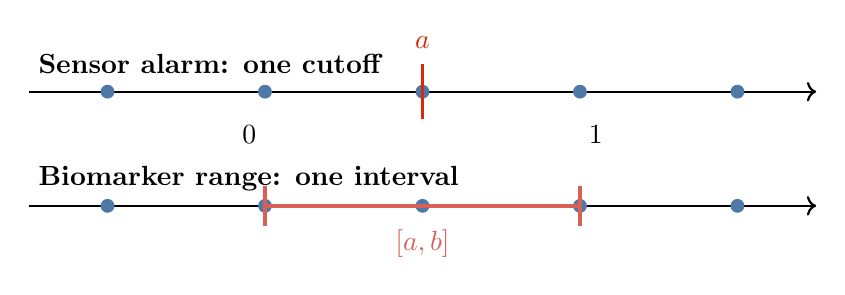
\begin{tikzpicture}[x=1.0cm,y=1cm]
    \node[anchor=west,font=\bfseries] at (0,1.35) {Sensor alarm: one cutoff};
    \draw[thick,->] (0,1)--(10,1);
    \foreach \x in {1,3,5,7,9}{\fill[pointblue] (\x,1) circle (2.5pt);}
    \draw[slideorange,very thick] (5,0.65)--(5,1.35);
    \node[slideorange,above=2pt] at (5,1.35) {$a$};
    \node at (2.8,0.45) {0};\node at (7.2,0.45) {1};
    \node[anchor=west,font=\bfseries] at (0,-0.10) {Biomarker range: one interval};
    \draw[thick,->] (0,-0.45)--(10,-0.45);
    \foreach \x in {1,3,5,7,9}{\fill[pointblue] (\x,-0.45) circle (2.5pt);}
    \draw[pointred,very thick] (3,-0.45)--(7,-0.45);
    \draw[pointred,very thick] (3,-0.70)--(3,-0.20);
    \draw[pointred,very thick] (7,-0.70)--(7,-0.20);
    \node[pointred,below=5pt] at (5,-0.45) {$[a,b]$};
  \end{tikzpicture}
  \end{center}
  \vspace{0.04cm}
  \centering
  Infinitely many parameter values can produce only finitely many behaviors on the observed points.
\end{frame}

\begin{frame}[t]{Restriction of a Class to a Sample}
  \vspace{0.04cm}
  For $S_X=(x_1,\ldots,x_m)$, define the set of prediction vectors
  \[
    \Hc\vert_{S_X}
    =\bigl\{(h(x_1),\ldots,h(x_m)):h\in\Hc\bigr\}.
  \]
  Even if $\Hc$ is infinite, $\Hc\vert_{S_X}$ is finite for binary-valued hypotheses:
  \[
    \abs{\Hc\vert_{S_X}}\le 2^m.
  \]
  \vspace{0.04cm}
  \begin{center}
  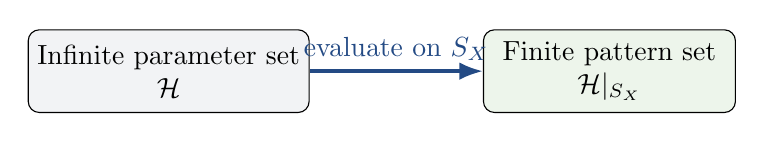
\begin{tikzpicture}[
      box/.style={draw=black,rounded corners=4pt,minimum width=3.2cm,minimum height=1.05cm,align=center,fill=softgray},
      arr/.style={-{Latex[length=3mm]},very thick,deepblue}
    ]
    \node[box] (inf) {Infinite parameter set\\$\Hc$};
    \node[box,right=2.2cm of inf,fill=softgreen] (pat) {Finite pattern set\\$\Hc\vert_{S_X}$};
    \draw[arr] (inf) -- node[above]{evaluate on $S_X$} (pat);
  \end{tikzpicture}
  \end{center}
\end{frame}

% ORIGINAL PDF SLIDE 30: Growth Function
\begin{frame}[t]{Growth Function}
  \vspace{0.04cm}
  For a binary hypothesis set $\Hc$, its growth function is
  \begin{beamercolorbox}[rounded=true,sep=0.20cm,wd=\linewidth]{block body}
    \[
      \boxed{
      \PiH(m)=
      \max_{x_1,\ldots,x_m\in\X}
      \abs{\bigl\{(h(x_1),\ldots,h(x_m)):h\in\Hc\bigr\}}.}
    \]
  \end{beamercolorbox}
  \vspace{0.15cm}
  \begin{itemize}
    \setlength{\itemsep}{0.10cm}
    \item $\PiH(m)$ is the maximum number of dichotomies realizable on $m$ points.
    \item Always $1\le\PiH(m)\le 2^m$.
    \item The maximum is over point placement, not over labels.
  \end{itemize}
\end{frame}

% ORIGINAL PDF SLIDE 31: Example: Thresholds on the Real Line
\begin{frame}[t]{Example: Thresholds on the Real Line}
  \vspace{0.02cm}
  Let
  \[
    \Hc_{\mathrm{thr}}=\{h_a(x)=\ind{x\ge a}:a\in\mathbb{R}\}.
  \]
  On $m$ ordered points $x_1<\cdots<x_m$, every labeling has the form
  \[
    00\cdots 0011\cdots 11.
  \]
  There are $m+1$ possible switch locations, so
  \[
    \boxed{\Pi_{\Hc_{\mathrm{thr}}}(m)=m+1.}
  \]
  \begin{center}
  \begin{tikzpicture}[scale=0.72]
    \draw[thick] (0,0)--(10,0);
    \foreach \x in {1,2.5,4,5.5,7,8.5}{\fill[pointblue] (\x,0) circle (2.6pt);}
    \draw[very thick,pointred] (4.7,-0.45)--(4.7,0.60) node[above] {$a$};
    \node at (2.8,-0.65) {$0$};
    \node at (6.8,-0.65) {$1$};
  \end{tikzpicture}
  \end{center}
\end{frame}

% ORIGINAL PDF SLIDE 32: Example: Intervals on the Real Line
\begin{frame}[t]{Example: Intervals on the Real Line}
  \vspace{0.03cm}
  Let $h_{a,b}(x)=\ind{a\le x\le b}$. On ordered points, the positive labels form one contiguous block.
  \vspace{0.05cm}
  \begin{itemize}
    \setlength{\itemsep}{0.12cm}
    \item One labeling is all negative.
    \item A nonempty positive block is determined by left and right endpoints.
  \end{itemize}
  Therefore,
  \[
    \boxed{
    \Pi_{\Hc_{\mathrm{int}}}(m)
    =1+\frac{m(m+1)}{2}.}
  \]
  \vspace{0.04cm}
  For $m=3$, this gives $7$: every labeling except $101$ is realizable.
\end{frame}

% ORIGINAL PDF SLIDE 33: Massart's Lemma
% MOTIVATION M07 -- before original PDF page 33: Massart's Lemma
\begin{frame}[t]{101 Vectors, Many Sign Draws}
  \vspace{0.04cm}
  \small

  Consider increasing thresholds on $100$ distinct ordered inputs.
  Encode their predictions as $-1$ and $+1$.
  \begin{center}
  \renewcommand{\arraystretch}{1.15}
  \begin{tabular}{lc}
    \toprule
    Quantity & Value\\
    \midrule
    Possible real cutoffs & infinitely many\\
    Distinct prediction vectors & $101$\\
    Euclidean norm of each prediction vector & $\sqrt{100}=10$\\
    Possible random sign vectors & $2^{100}\approx1.27\times10^{30}$\\
    \bottomrule
  \end{tabular}
  \end{center}
  Exact averaging over all sign vectors is impractical even in this example.
  \vspace{0.15cm}
  \KeyBox{Can the number of prediction vectors and their Euclidean norms
  bound their best average correlation with random signs?}

\end{frame}

\begin{frame}[t]{Massart's Lemma}
  \vspace{0.03cm}
  Let $A\subset\mathbb{R}^m$ be finite and let
  $r=\max_{a\in A}\norm{a}_2$. Then
  \begin{beamercolorbox}[rounded=true,sep=0.20cm,wd=\linewidth]{block body}
    \[
      \boxed{
      \E_\sigma\left[
        \sup_{a\in A}\frac1m\angles{\sigma,a}
      \right]
      \le \frac{r\sqrt{2\log\abs{A}}}{m}.}
    \]
  \end{beamercolorbox}
  \vspace{0.15cm}
  \begin{itemize}
    \setlength{\itemsep}{0.10cm}
    \item Complexity depends logarithmically on the number of candidate vectors.
    \item The Euclidean radius $r$ controls their scale.
    \item We apply the lemma to evaluation vectors of hypotheses.
  \end{itemize}
  \SourceNote{Massart (2000); proof route follows the chapter's exponential-moment argument.}
\end{frame}

% ORIGINAL PDF SLIDE 34: Massart's Lemma: Exponential-Moment Step
\begin{frame}[t]{Massart's Lemma: Exponential-Moment Step}
  \vspace{0.01cm}
  {\small
  For any $\lambda>0$, Jensen's inequality and the union bound give
  \begin{align*}
    \exp\!\left(\lambda\E_\sigma\sup_{a\in A}\angles{\sigma,a}\right)
    &\le \E_\sigma\exp\!\left(\lambda\sup_{a\in A}\angles{\sigma,a}\right)\le \sum_{a\in A}\E_\sigma e^{\lambda\angles{\sigma,a}}.
  \end{align*}
  Independence and Hoeffding's lemma imply
  \begin{align*}
    \E_\sigma e^{\lambda\angles{\sigma,a}}
    &=\prod_{i=1}^m\E e^{\lambda\sigma_i a_i}
    \le \exp\!\left(\frac{\lambda^2\norm{a}_2^2}{2}\right)\le \exp\!\left(\frac{\lambda^2r^2}{2}\right).
  \end{align*}}
\end{frame}

% ORIGINAL PDF SLIDE 35: Massart's Lemma: Optimize the Parameter
\begin{frame}[t]{Massart's Lemma: Optimize the Parameter}
  \vspace{0.03cm}
  Taking logarithms gives
  \[
    \E_\sigma\sup_{a\in A}\angles{\sigma,a}
    \le \frac{\log\abs{A}}{\lambda}+\frac{\lambda r^2}{2}.
  \]
  Choose
  \[
    \lambda=\frac{\sqrt{2\log\abs{A}}}{r}\quad\text{if }r>0,\ \abs{A}>1
  \]
  to balance the terms. Then
  \[
    \E_\sigma\sup_{a\in A}\angles{\sigma,a}
    \le r\sqrt{2\log\abs{A}}.
  \]
  Dividing by $m$ proves the result. If $r=0$ or $\abs{A}=1$, both sides are zero.
  \vspace{0.08cm}
  \KeyBox{A square root of a logarithm emerges from optimizing an exponential-moment bound.}
\end{frame}

% ORIGINAL PDF SLIDE 36: Growth Function Bounds Rademacher Complexity
\begin{frame}[t]{Growth Function Bounds Rademacher Complexity}
  \vspace{0.01cm}
  For binary functions $h:\X\to\pmone$, each evaluation vector has norm $\sqrt m$. On any fixed sample,
  \[
    \abs{\Hc\vert_{S_X}}\le\PiH(m).
  \]
  Massart's lemma gives
  \[
    \RadS(\Hc)
    \le \sqrt{\frac{2\log\abs{\Hc\vert_{S_X}}}{m}}
    \le \sqrt{\frac{2\log\PiH(m)}{m}}.
  \]
  Averaging over samples preserves the bound:
  \begin{beamercolorbox}[rounded=true,sep=0.18cm,wd=\linewidth]{block body}
    \[
      \boxed{\Rad_m(\Hc)\le\sqrt{\frac{2\log\PiH(m)}{m}}.}
    \]
  \end{beamercolorbox}
\end{frame}

% ORIGINAL PDF SLIDE 37: Generalization Bound via Growth Function
\begin{frame}[t]{Generalization Bound via Growth Function}
  \vspace{0.04cm}
  Combining the binary Rademacher bound with the growth estimate yields: with probability at least $1-\delta$, every $h\in\Hc$ satisfies
  \begin{beamercolorbox}[rounded=true,sep=0.20cm,wd=\linewidth]{block body}
    \[
      \boxed{
      R(h)
      \le \Rhat(h)
      +\sqrt{\frac{2\log\PiH(m)}{m}}
      +\sqrt{\frac{\log(1/\delta)}{2m}}.}
    \]
  \end{beamercolorbox}
  \vspace{0.15cm}
  \begin{itemize}
    \setlength{\itemsep}{0.10cm}
    \item We replaced $\log\abs{\Hc}$ by $\log\PiH(m)$.
    \item This remains finite for every binary class on a finite sample.
    \item We still need a practical way to bound $\PiH(m)$ for all $m$.
  \end{itemize}
\end{frame}

% ORIGINAL PDF SLIDE 38: VC Dimension
\SectionSlide{VC Dimension}{}

% ORIGINAL PDF SLIDE 39: Shattering and VC Dimension
% MOTIVATION M08 -- before original PDF page 39: Shattering and VC Dimension
\begin{frame}[t]{An Interval Labeling Game}
  \vspace{0.04cm}
  \small

  A classifier predicts $1$ inside one interval and $0$ outside. Think of
  $x$ as a biomarker or dosage level and the interval as a target range.
  Imagine that someone chooses the labels \emph{after} we place the points.
  \begin{center}
  \renewcommand{\arraystretch}{1.15}
  \begin{tabular}{lll}
    \toprule
    Inputs & Labels to fit & Can one interval fit them?\\
    \midrule
    $x_1<x_2$ & $00,01,10,11$ & Yes, all four choices\\
    $x_1<x_2<x_3$ & $010$ & Yes, keep only the middle point\\
    $x_1<x_2<x_3$ & $101$ & No, an interval cannot skip the middle\\
    \bottomrule
  \end{tabular}
  \end{center}
  The labeling $010$ is feasible. Our challenge is to fit
  \emph{every} labeling of the same points.
  \vspace{0.20cm}
  \KeyBox{What is the largest number of points for which our class can win
  against every possible choice of labels?}

\end{frame}

% MOTIVATION V04 -- before original PDF page 39: Shattering and VC Dimension
\begin{frame}[t]{Shattering as a Labeling Game}
  \vspace{0.04cm}\small
  Place the points first. Then ask whether the class can answer every labeling challenge.
  \begin{columns}[T,totalwidth=\textwidth]
    \begin{column}{0.52\textwidth}
      \textbf{Two points: all four challenges}
      \begin{center}
      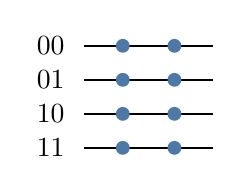
\begin{tikzpicture}[x=0.82cm,y=0.48cm]
        \foreach \y/\l in {3.0/00,2.1/01,1.2/10,0.3/11}{
          \node[anchor=east] at (-0.15,\y) {$\l$};
          \draw[thick] (0,\y)--(2,\y);
          \fill[pointblue] (0.6,\y) circle (2.5pt);
          \fill[pointblue] (1.4,\y) circle (2.5pt);
        }
      \end{tikzpicture}
      \end{center}
      Every labeling can be realized by a suitable interval.
    \end{column}
    \begin{column}{0.44\textwidth}
      \textbf{Three points: one challenge fails}
      \begin{center}
      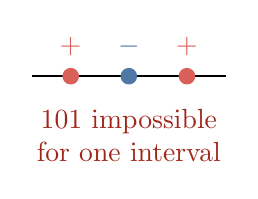
\begin{tikzpicture}[x=0.82cm]
        \draw[thick] (0,0)--(3,0);
        \fill[pointred] (0.6,0) circle (3pt) node[above=4pt] {$+$};
        \fill[pointblue] (1.5,0) circle (3pt) node[above=4pt] {$-$};
        \fill[pointred] (2.4,0) circle (3pt) node[above=4pt] {$+$};
        \node[darkred,align=center] at (1.5,-0.75) {$101$ impossible\\for one interval};
      \end{tikzpicture}
      \end{center}
    \end{column}
  \end{columns}
  \KeyBox{The largest number of points on which every labeling is possible is the VC dimension.}
\end{frame}

\begin{frame}[t]{Shattering and VC Dimension}
  \vspace{0.04cm}
  A set $S_X=\{x_1,\ldots,x_m\}$ is \textbf{shattered} by $\Hc$ if
  \[
    \abs{\Hc\vert_{S_X}}=2^m.
  \]
  The VC dimension is
  \begin{beamercolorbox}[rounded=true,sep=0.20cm,wd=\linewidth]{block body}
    \[
      \boxed{
      \vcdim(\Hc)=\sup\{m\ge0:\PiH(m)=2^m\}.}
    \]
  \end{beamercolorbox}
  \vspace{0.15cm}
  \begin{itemize}
    \setlength{\itemsep}{0.10cm}
    \item If arbitrarily large finite sets are shattered, $\vcdim(\Hc)=\infty$.
    \item Infinite cardinality does not imply infinite VC dimension.
    \item Finite VC dimension means complete freedom eventually stops.
  \end{itemize}
\end{frame}

% ORIGINAL PDF SLIDE 40: How to Prove a VC-Dimension Claim
\begin{frame}[t]{How to Prove a VC-Dimension Claim}
  \vspace{0.05cm}
  To show $\vcdim(\Hc)=d$, prove two statements:
  \vspace{0.05cm}
  \begin{enumerate}
    \setlength{\itemsep}{0.18cm}
    \item \textbf{Lower bound:} exhibit one set of $d$ points that $\Hc$ shatters.
    \item \textbf{Upper bound:} prove that no set of $d+1$ points can be shattered.
  \end{enumerate}
  \vspace{0.10cm}
  \begin{columns}[T,totalwidth=\textwidth]
    \begin{column}{0.48\textwidth}
      \KeyBox{Lower bounds are constructive: find a favorable configuration.}
    \end{column}
    \begin{column}{0.48\textwidth}
      \OrangeBox{Upper bounds are universal: rule out every configuration.}
    \end{column}
  \end{columns}
  \vspace{0.12cm}
  A common mistake is to show only that one particular set of $d+1$ points is not shattered.
\end{frame}

% ORIGINAL PDF SLIDE 41: VC Dimension of Thresholds: $1$
\begin{frame}[t]{VC Dimension of Thresholds: $1$}
  \vspace{0.05cm}
  For $h_a(x)=\ind{x\ge a}$:
  \begin{itemize}
    \setlength{\itemsep}{0.14cm}
    \item One point can receive either label by moving the threshold.
    \item For two ordered points $x_1<x_2$, the labeling $(1,0)$ is impossible.
  \end{itemize}
  Therefore,
  \[
    \boxed{\vcdim(\Hc_{\mathrm{thr}})=1.}
  \]
  \begin{center}
  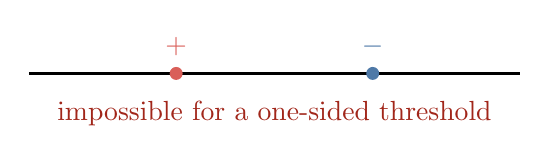
\begin{tikzpicture}[scale=0.78]
    \draw[thick] (0,0)--(8,0);
    \fill[pointred] (2.4,0) circle (3pt) node[above=3pt] {$+$};
    \fill[pointblue] (5.6,0) circle (3pt) node[above=3pt] {$-$};
    \node[darkred] at (4,-0.65) {impossible for a one-sided threshold};
  \end{tikzpicture}
  \end{center}
\end{frame}

% ORIGINAL PDF SLIDE 42: VC Dimension of Intervals: $2$
\begin{frame}[t]{VC Dimension of Intervals: $2$}
  \vspace{0.01cm}
  \textbf{Lower bound.} Any two points can realize all four labelings using an interval: empty, left only, right only, or both.
  \vspace{0.08cm}
  \textbf{Upper bound.} For three ordered points $x_1<x_2<x_3$, the labeling
  \[
    (+,-,+)
  \]
  is impossible because the positive region of an interval is contiguous.
  \vspace{0.05cm}
  \[
    \boxed{\vcdim(\Hc_{\mathrm{int}})=2.}
  \]
  \begin{center}
  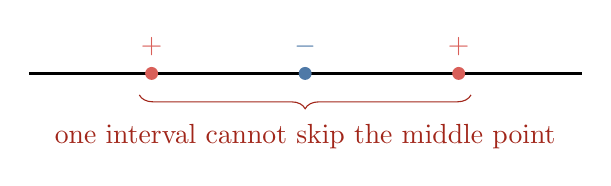
\begin{tikzpicture}[scale=0.78]
    \draw[thick] (0,0)--(9,0);
    \fill[pointred] (2,0) circle (3pt) node[above=3pt] {$+$};
    \fill[pointblue] (4.5,0) circle (3pt) node[above=3pt] {$-$};
    \fill[pointred] (7,0) circle (3pt) node[above=3pt] {$+$};
    \draw[darkred,decorate,decoration={brace,amplitude=5pt,mirror}] (1.8,-0.35)--(7.2,-0.35)
       node[midway,below=7pt] {one interval cannot skip the middle point};
  \end{tikzpicture}
  \end{center}
\end{frame}

% ORIGINAL PDF SLIDE 43: Axis-Aligned Rectangles in $\mathbb{R}^2$: VC Dimension $4$
\begin{frame}[t]{Axis-Aligned Rectangles in $\mathbb{R}^2$: VC Dimension $4$}
  \vspace{0.01cm}
  \begin{columns}[T,totalwidth=\textwidth]
    \begin{column}{0.46\textwidth}
      \begin{center}
      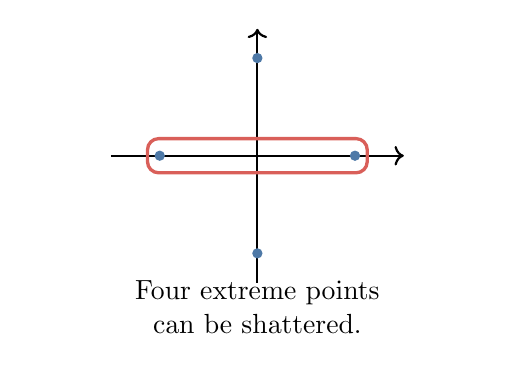
\begin{tikzpicture}[scale=0.62]
        \draw[->,thick] (-3,0)--(3,0);
        \draw[->,thick] (0,-2.6)--(0,2.6);
        \fill[pointblue] (-2,0) circle (3pt);
        \fill[pointblue] (2,0) circle (3pt);
        \fill[pointblue] (0,2) circle (3pt);
        \fill[pointblue] (0,-2) circle (3pt);
        \draw[pointred,very thick,rounded corners] (-2.25,-0.35) rectangle (2.25,0.35);
        \node[text width=5.6cm,align=center] at (0,-3.1) {Four extreme points can be shattered.};
      \end{tikzpicture}
      \end{center}
    \end{column}
    \begin{column}{0.52\textwidth}
      {\small
      \begin{itemize}
        \setlength{\itemsep}{0.10cm}
        \item Lower bound: use left, right, top, and bottom extremes.
        \item Upper bound: select one point attaining each coordinate minimum or maximum (at most four points).
        \item Label the selected points positive and one unselected point negative.
        \item A rectangle containing the selected points must contain the unselected point.
      \end{itemize}}
    \end{column}
  \end{columns}
  \vspace{0.01cm}
  \[
    \boxed{\vcdim(\text{axis-aligned rectangles in }\mathbb{R}^2)=4.}
  \]
\end{frame}



\begin{frame}[t]{Linear Separators in $\mathbb{R}^2$: VC Dimension $3$}
  \vspace{0.01cm}
  \begin{columns}[T,totalwidth=\textwidth]
    \begin{column}{0.46\textwidth}
      \textbf{Lower bound}
      \begin{center}
      \begin{tikzpicture}[scale=0.65]
        \fill[pointblue] (0,0) circle (3pt);
        \fill[pointblue] (3.5,0.3) circle (3pt);
        \fill[pointblue] (1.5,2.7) circle (3pt);
        \draw[deepblue,dashed] (-0.5,1.1)--(4,2.1);
        \node[text width=6cm,align=center] at (1.8,-0.7) {Three non-collinear points};
      \end{tikzpicture}
      \end{center}
      Every dichotomy is linearly separable.
    \end{column}
    \begin{column}{0.52\textwidth}
      \textbf{Upper bound}
      \begin{itemize}
        \setlength{\itemsep}{0.10cm}
        \item Four points in convex position admit an XOR labeling that no line separates.
        \item Otherwise, one point lies in the convex hull of the others (possibly on its boundary). Label that point positive and the others negative.
      \end{itemize}
    \end{column}
  \end{columns}
  \vspace{0.04cm}
  \[
    \boxed{\vcdim(\text{affine halfspaces in }\mathbb{R}^2)=3.}
  \]
\end{frame}

% ORIGINAL PDF SLIDE 45: Hyperplanes in $\mathbb{R}^d$: VC Dimension $d+1$
\begin{frame}[t]{Hyperplanes in $\mathbb{R}^d$: VC Dimension $d+1$}
  \vspace{0.01cm}
  Consider affine classifiers
  \[
    h_{w,b}(x)=\sign(w^Tx+b).
  \]
  \begin{itemize}
    \setlength{\itemsep}{0.12cm}
    \item \textbf{Lower bound:} $d+1$ affinely independent points can be shattered.
    \item \textbf{Upper bound:} any $d+2$ points are affinely dependent, forcing at least one nonseparable dichotomy.
  \end{itemize}
  \vspace{0.05cm}
  \begin{beamercolorbox}[rounded=true,sep=0.18cm,wd=\linewidth]{block body}
    \[
      \boxed{\vcdim(\text{affine halfspaces in }\mathbb{R}^d)=d+1.}
    \]
  \end{beamercolorbox}
  \vspace{0.08cm}
  \centering
  The proof is geometric; parameter counting alone is not a general VC-dimension argument.
\end{frame}

% ORIGINAL PDF SLIDE 46: Finite and Infinite VC Dimension
\begin{frame}[t]{Finite and Infinite VC Dimension}
  \vspace{0.01cm}
  \begin{itemize}
    \setlength{\itemsep}{0.10cm}
    \item Convex polygons in $\mathbb{R}^2$ with at most $d\ge3$ sides have $\vcdim=2d+1$.
    \item The class of all convex polygons has infinite VC dimension.
  \end{itemize}
  \begin{center}
  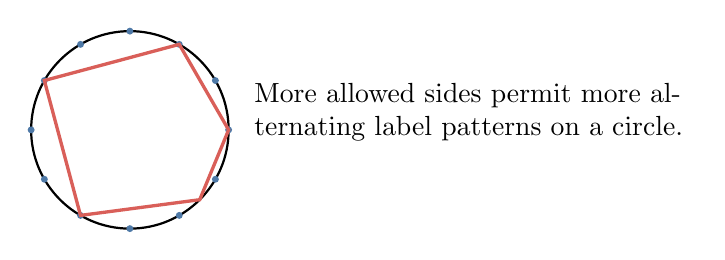
\begin{tikzpicture}[scale=0.57]
    \draw[thick] (0,0) circle (2.2cm);
    \foreach \a in {0,30,...,330}{
      \fill[pointblue] ({2.2*cos(\a)},{2.2*sin(\a)}) circle (2.2pt);
    }
    \draw[pointred,very thick] (0:2.2) -- (60:2.2) -- (150:2.2) -- (240:2.2) -- (315:2.2) -- cycle;
    \node[align=left,text width=5.5cm] at (7.6,0.4) {More allowed sides permit more alternating label patterns on a circle.};
  \end{tikzpicture}
  \end{center}
  \vspace{0.02cm}
  \OrangeBox{Infinite VC dimension means arbitrarily large finite sets can be shattered; it is stronger than having infinitely many hypotheses.}
\end{frame}



% ORIGINAL PDF SLIDE 48: Sauer's Lemma
% MOTIVATION M09 -- before original PDF page 48: Sauer's Lemma
\begin{frame}[t]{Counting Interval Patterns}
  \vspace{0.04cm}
  \small

  Intervals cannot fit $101$ on three ordered inputs. Their positive labels
  must form one contiguous block, giving $1+m(m+1)/2$ patterns.
  \begin{center}
  \renewcommand{\arraystretch}{1.15}
  \begin{tabular}{r r r}
    \toprule
    Number of inputs $m$ & Interval patterns & All binary patterns $2^m$\\
    \midrule
    3 & 7 & 8\\
    5 & 16 & 32\\
    10 & 56 & 1,024\\
    20 & 211 & 1,048,576\\
    \bottomrule
  \end{tabular}
  \end{center}
  Missing one pattern on every triple accompanies a large restriction on
  longer label sequences.
  \vspace{0.15cm}
  \KeyBox{If a different class also has VC dimension $2$, must it obey a
  similar bound even without the geometry of intervals?}

\end{frame}

\begin{frame}[t]{Sauer's Lemma}
  \vspace{0.04cm}
  If $\vcdim(\Hc)=d$, then for every $m\in\mathbb{N}$,
  \begin{beamercolorbox}[rounded=true,sep=0.22cm,wd=\linewidth]{block body}
    \[
      \boxed{
      \PiH(m)\le\sum_{i=0}^{d}\binom{m}{i}.}
    \]
  \end{beamercolorbox}
  \vspace{0.15cm}
  This transforms a local shattering restriction into a global bound on dichotomies.
  \vspace{0.10cm}
  \begin{itemize}
    \setlength{\itemsep}{0.10cm}
    \item For $m\le d$, the right side equals $2^m$.
    \item For fixed $d$, it grows polynomially as $m$ increases.
  \end{itemize}
  \SourceNote{Vapnik--Chervonenkis; Sauer; also independently Shelah.}
\end{frame}

% ORIGINAL PDF SLIDE 49: Sauer's Lemma: Proof Setup
% MOTIVATION M10 -- before original PDF page 49: Sauer's Lemma: Proof Setup
\begin{frame}[t]{Extending a Prediction Pattern}
  \vspace{0.04cm}
  \small

  Increasing thresholds on $x_1<x_2<x_3$ produce
  \[
    G=\{000,001,011,111\}.
  \]
  Remove the last coordinate and group the remaining prefixes.
  \begin{center}
  \renewcommand{\arraystretch}{1.15}
  \begin{tabular}{ccc}
    \toprule
    Prefix on $(x_1,x_2)$ & Allowed last labels & Full patterns\\
    \midrule
    $00$ & $0$ or $1$ & $000,001$\\
    $01$ & $1$ & $011$\\
    $11$ & $1$ & $111$\\
    \bottomrule
  \end{tabular}
  \end{center}
  There are three prefixes, and one prefix has an extra extension:
  \[
    4=3+1.
  \]
  \KeyBox{Count each prefix once, then add the prefixes that allow both
  labels at the last point. This is the split used in Sauer's proof.}

\end{frame}

\begin{frame}[t]{Sauer's Lemma: Proof Setup}
  \vspace{0.01cm}
  Fix $S=\{x_1,\ldots,x_m\}$ on which $\Hc$ realizes the maximum number of patterns, and let
  \[
    G=\Hc\vert_S.
  \]
  Remove the last point and write $S'=S\setminus\{x_m\}$. Define
  \begin{align*}
    G_1&=\{g\vert_{S'}:g\in G\},\\
    G_2&=\{u:\text{$u$ occurs in $G$ with both labels at $x_m$}\}.
  \end{align*}
  \vspace{0.02cm}
  \begin{beamercolorbox}[rounded=true,sep=0.16cm,wd=\linewidth]{alertblock body}
    Every pattern in $G_1$ contributes once to $G$; patterns in $G_2$ contribute one extra copy. Hence
    \[
      \abs{G}=\abs{G_1}+\abs{G_2}.
    \]
  \end{beamercolorbox}
\end{frame}

% ORIGINAL PDF SLIDE 50: Sauer's Lemma: The Key Recurrence
\begin{frame}[t]{Sauer's Lemma: The Key Recurrence}
  \vspace{0.03cm}
  The two restricted families have smaller parameters:
  \begin{itemize}
    \setlength{\itemsep}{0.15cm}
    \item $G_1$ lives on $m-1$ points and has VC dimension at most $d$.
    \item $G_2$ has VC dimension at most $d-1$; otherwise a set shattered by $G_2$, together with $x_m$, would give $d+1$ shattered points.
  \end{itemize}
  Therefore the extremal growth quantity satisfies
  \[
    \Pi_d(m)
    \le \Pi_d(m-1)+\Pi_{d-1}(m-1).
  \]
  \vspace{0.08cm}
  \KeyBox{The recurrence mirrors Pascal's identity for binomial coefficients.}
\end{frame}

% ORIGINAL PDF SLIDE 51: Sauer's Lemma: Close the Induction
\begin{frame}[t]{Sauer's Lemma: Close the Induction}
  \vspace{-0.02cm}
  {\small
  Apply the induction hypothesis to the recurrence:
  \begin{align*}
    \Pi_d(m)
    &\le \sum_{i=0}^{d}\binom{m-1}{i}
      +\sum_{i=0}^{d-1}\binom{m-1}{i}\\
    &=\sum_{i=0}^{d}
      \left[\binom{m-1}{i}+\binom{m-1}{i-1}\right]\\
    &=\sum_{i=0}^{d}\binom{m}{i}.
  \end{align*}
  The boundary cases $d=0$ and $m=1$ are immediate.}
  \vspace{0.02cm}
  \OrangeBox{\small The proof tracks which restrictions can branch into both labels at the final point.}
\end{frame}

% ORIGINAL PDF SLIDE 52: Polynomial Growth Consequence
\begin{frame}[t]{Polynomial Growth Consequence}
  \vspace{0.02cm}
  For $m\ge d\ge1$,
  \[
    \sum_{i=0}^{d}\binom{m}{i}
    \le \left(\frac{em}{d}\right)^d.
  \]
  Therefore,
  \begin{beamercolorbox}[rounded=true,sep=0.20cm,wd=\linewidth]{block body}
    \[
      \boxed{
      \PiH(m)\le\left(\frac{em}{d}\right)^d=O(m^d).}
    \]
  \end{beamercolorbox}
  \vspace{0.14cm}
  Taking logarithms gives
  \[
    \log\PiH(m)\le d\log\!\left(\frac{em}{d}\right).
  \]
  This is exactly the quantity needed in the growth-function bound.
\end{frame}

% ORIGINAL PDF SLIDE 53: The Growth Dichotomy
\begin{frame}[t]{The Growth Dichotomy}
  \vspace{0.04cm}
  A binary hypothesis class has one of two qualitatively different behaviors:
  \vspace{0.08cm}
  \begin{columns}[T,totalwidth=\textwidth]
    \begin{column}{0.48\textwidth}
      \KeyBox{
      \centering
      \textbf{Finite VC dimension $d$}\\[0.10cm]
      $\PiH(m)=O(m^d)$\\
      polynomial growth}
    \end{column}
    \begin{column}{0.48\textwidth}
      \OrangeBox{
      \centering
      \textbf{Infinite VC dimension}\\[0.10cm]
      $\PiH(m)=2^m$ for every $m$\\
      maximal exponential growth}
    \end{column}
  \end{columns}
  \vspace{0.18cm}
  \centering
  There is no intermediate asymptotic regime for the worst-case growth function.
\end{frame}

% ORIGINAL PDF SLIDE 54: VC Generalization Bound via Rademacher Complexity
\begin{frame}[t]{VC Generalization Bound via Rademacher Complexity}
  \vspace{0.02cm}
  Let $\Hc\subseteq\{h:\X\to\pmone\}$ have VC dimension $d$, with $m\ge d\ge1$. Combining Sauer's lemma with the Rademacher bound gives, with probability at least $1-\delta$, for all $h\in\Hc$,
  \begin{beamercolorbox}[rounded=true,sep=0.18cm,wd=\linewidth]{block body}
    \[
      \boxed{
      R(h)\le\Rhat(h)
      +\sqrt{\frac{2d\log(em/d)}{m}}
      +\sqrt{\frac{\log(1/\delta)}{2m}}.}
    \]
  \end{beamercolorbox}
  \vspace{0.10cm}
  Up to logarithmic factors, the estimation term behaves like
  \[
    \sqrt{\frac{d+\log(1/\delta)}{m}}.
  \]
\end{frame}

% ORIGINAL PDF SLIDE 55: The Standard VC Bound
\begin{frame}[t]{The Standard VC Bound}
  \vspace{0.02cm}
  For $m\ge d\ge1$, a direct symmetrization and growth-function argument gives another classical form. With probability at least $1-\delta$, for all $h\in\Hc$,
  \begin{beamercolorbox}[rounded=true,sep=0.18cm,wd=\linewidth]{block body}
    \[
      \boxed{
      R(h)\le\Rhat(h)
      +\sqrt{
        \frac{8d\log(2em/d)+8\log(4/\delta)}{m}
      }.}
    \]
  \end{beamercolorbox}
  \vspace{0.10cm}
  It follows from a tail inequality of the form
  \[
    \Prb\!\left(\sup_{h\in\Hc}\abs{R(h)-\Rhat(h)}>\eps\right)
    \le 4\PiH(2m)e^{-m\eps^2/8}.
  \]
  \SourceNote{Classical Vapnik--Chervonenkis bound, as compared in Chapter 3.}
\end{frame}

% ORIGINAL PDF SLIDE 56: Comparing the Two Upper Bounds
\begin{frame}[t]{Comparing the Two Upper Bounds}
  \vspace{0.01cm}
  {\small
  \renewcommand{\arraystretch}{1.17}
  \begin{center}
  \begin{tabular}{p{2.55cm}p{4.15cm}p{4.15cm}}
    \toprule
     & \textbf{Rademacher route} & \textbf{Classical VC route}\\
    \midrule
    Main object & $\Rad_m(\Hc)$ or $\RadS(\Hc)$ & $\PiH(2m)$ and $d$\\
    Data dependence & Possible & No\\
    Typical scale & $\sqrt{d\log(m/d)/m}$ & $\sqrt{d\log(m/d)/m}$\\
    Strength & Flexible for real-valued and structured classes & Clean distribution-free binary result\\
    Limitation & May be hard to compute & A single integer may be coarse\\
    \bottomrule
  \end{tabular}
  \end{center}}
  \vspace{0.08cm}
  \KeyBox{\small\raggedright VC dimension controls worst-case capacity; empirical complexity can reveal easier data.\par}
\end{frame}


\begin{frame}[t]{Sample Complexity from the VC Bound}
  \vspace{-0.04cm}
  {\footnotesize
  To make the uniform gap at most $\eps$, it suffices that
  \[
    \sqrt{\frac{d\log(m/d)+\log(1/\delta)}{m}}
    \lesssim\eps.
  \]
  Solving the implicit logarithm yields
  \begin{beamercolorbox}[rounded=true,sep=0.10cm,wd=\linewidth]{block body}
    \[
      \boxed{
      m=O\!\left(
        \frac{d\log(1/\eps)+\log(1/\delta)}{\eps^2}
      \right)}
    \]
    for agnostic uniform convergence.
  \end{beamercolorbox}
  \vspace{0.02cm}
  \begin{itemize}
    \setlength{\itemsep}{0.03cm}
    \item Linear dependence on capacity $d$ up to a logarithm.
    \item Quadratic dependence on target accuracy $1/\eps$.
    \item Logarithmic dependence on confidence $1/\delta$.
  \end{itemize}}
\end{frame}

% ORIGINAL PDF SLIDE 58: Worked Example: Intervals
\begin{frame}[t]{Worked Example: Intervals}
  \vspace{0.01cm}
  For intervals on $\mathbb{R}$, $d=2$. Take $m=5000$ and $\delta=0.05$. The Rademacher--VC deviation term is
  \begin{align*}
    &\sqrt{\frac{2d\log(em/d)}{m}}
      +\sqrt{\frac{\log(1/\delta)}{2m}}\\
    &\quad=\sqrt{\frac{4\log(2500e)}{5000}}
      +\sqrt{\frac{\log 20}{10000}}\\
    &\quad\approx 0.101.
  \end{align*}
  Thus, simultaneously for all intervals,
  \[
    R(h)\lesssim \Rhat(h)+0.101.
  \]
  \vspace{0.04cm}
  \OrangeBox{The theorem is distribution-free and uniform, so it is often conservative compared with test-set estimates.}
\end{frame}

% ORIGINAL PDF SLIDE 59: Worked Example: Linear Separators
\begin{frame}[t]{Worked Example: Linear Separators}
  \vspace{0.01cm}
  Affine halfspaces in $\mathbb{R}^{20}$ have $d=21$. With $m=5000$ and $\delta=0.05$,
  \[
    \sqrt{\frac{2d\log(em/d)}{m}}
    +\sqrt{\frac{\log(1/\delta)}{2m}}
    \approx 0.250.
  \]
  \begin{itemize}
    \setlength{\itemsep}{0.12cm}
    \item Capacity grows linearly with the model dimension.
    \item The bound is distribution-free, so it possibly ignores margin information and observed-sample geometry.
  \end{itemize}
  \vspace{0.06cm}
  \KeyBox{Capacity measures should match the algorithm and structure one wants to exploit.}
\end{frame}

% ORIGINAL PDF SLIDE 60: Lower Bounds
\SectionSlide{Lower Bounds}{}

% ORIGINAL PDF SLIDE 61: Lower Bound: Realizable Case
% MOTIVATION M12 -- before original PDF page 61: Lower Bound: Realizable Case
\begin{frame}[t]{Unseen Labels}
  \vspace{0.04cm}
  \small

  Suppose $\Hc$ shatters four inputs $\{a,b,c,d\}$. Choose a target
  uniformly from the $16$ possible labelings on these inputs.
  \begin{center}
  \renewcommand{\arraystretch}{1.15}
  \begin{tabular}{lcccc}
    \toprule
    Input & $a$ & $b$ & $c$ & $d$\\
    \midrule
    Observed in training? & Yes & Yes & No & No\\
    Observed label & $+$ & $-$ & ? & ?\\
    \bottomrule
  \end{tabular}
  \end{center}
  The four possibilities for the unseen pair are
  \[
    (y_c,y_d)\in\{(+,+),(+,-),(-,+),(-,-)\}.
  \]
  All remain equally likely. Whatever the learner predicts, its expected
  error on each unseen input is $1/2$ under this random target.
  \vspace{0.16cm}
  \KeyBox{Even a perfect fit to observed labels cannot determine unseen
  labels. Assigning probability mass to rarely seen inputs creates a
  lower bound that applies to every learning algorithm.}

\end{frame}

\begin{frame}[t]{Lower Bound: Realizable Case}
  \vspace{0.01cm}
  Let $\Hc$ have VC dimension $d>1$ and let $m\ge d$. For any learning algorithm $A$, there exist a distribution $\D$ and target $f\in\Hc$ such that
  \begin{beamercolorbox}[rounded=true,sep=0.18cm,wd=\linewidth]{alertblock body}
    \[
      \boxed{
      \Prb_{S\sim\D^m}\!\left[
        R_\D(h_S,f)>\frac{d-1}{32m}
      \right]\ge\frac{1}{100}.}
    \]
  \end{beamercolorbox}
  \vspace{0.10cm}
  Consequence for constant confidence:
  \[
    m=\Omega\!\left(\frac{d}{\eps}\right)
  \]
  examples are unavoidable in the realizable setting.
  \SourceNote{Ehrenfeucht, Haussler, Kearns, and Valiant (1988); Chapter 3 lower-bound theorem.}
\end{frame}

% ORIGINAL PDF SLIDE 62: Hard Distribution Intuition
\begin{frame}[t]{Hard Distribution Intuition}
  \vspace{0.01cm}
  Start with $d$ points shattered by $\Hc$:
  \[
    X_0=\{x_0,x_1,\ldots,x_{d-1}\}.
  \]
  Construct a distribution with
  \begin{itemize}
    \setlength{\itemsep}{0.12cm}
    \item most mass on an easy point $x_0$;
    \item small, equal masses on the other $d-1$ points;
    \item a target chosen from all labelings of those points.
  \end{itemize}
  \vspace{0.05cm}
  If the sample contains few rare points, many labels remain unseen. Because the set is shattered, those labels are unconstrained by observed data.
  \vspace{0.06cm}
  \OrangeBox{On an unseen rare point, any algorithm is effectively guessing a fair coin under a random target labeling.}
\end{frame}



% ORIGINAL PDF SLIDE 65: What the Three Complexity Measures Tell Us
\begin{frame}[t]{What the Three Complexity Measures Tell Us}
  \vspace{0.01cm}
  {\scriptsize
  \renewcommand{\arraystretch}{1.12}
  \begin{center}
  \begin{tabular}{p{2.35cm}p{2.95cm}p{3.05cm}p{3.05cm}}
    \toprule
    & \textbf{Rademacher} & \textbf{Growth function} & \textbf{VC dimension}\\
    \midrule
    Measures & noise fitting & number of dichotomies & largest shattered set\\
    Depends on & sample / distribution & worst $m$-point set & class only\\
    Applies to & real-valued classes & binary classes & binary classes\\
    Main use & sharp upper bounds & bridge to counting & upper and lower rates\\
    Output & $\RadS(\Gc)$ & $\PiH(m)$ & integer $d$\\
    \bottomrule
  \end{tabular}
  \end{center}}
  \vspace{0.06cm}
  \KeyBox{\small 
  \[
    \text{VC dimension}\Rightarrow\text{growth bound}\Rightarrow\text{Rademacher bound}\Rightarrow\text{generalization}.
  \]
  }
\end{frame}

% ORIGINAL PDF SLIDE 66: References and Questions
\begin{frame}[t]{References and Questions}
  \vspace{0.01cm}
  {\small
  \begin{itemize}
    \setlength{\itemsep}{0.07cm}
    \item M. Mohri, A. Rostamizadeh, and A. Talwalkar. \emph{Foundations of Machine Learning}, 2nd ed., Chapter 3. MIT Press, 2018.
    \item P. Massart. ``Some Applications of Concentration Inequalities to Statistics,'' 2000.
    \item V. Koltchinskii and D. Panchenko. ``Empirical Margin Distributions and Bounding the Generalization Error of Combined Classifiers,'' 2002.
    \item V. Vapnik and A. Chervonenkis; N. Sauer. Foundational growth-function and VC-dimension results.
    \item A. Ehrenfeucht, D. Haussler, M. Kearns, and L. Valiant. Realizable lower bound, 1988.
    \item M. Anthony and P. Bartlett. \emph{Neural Network Learning: Theoretical Foundations}, 1999.
  \end{itemize}}
  \vspace{0.10cm}
  \begin{beamercolorbox}[rounded=true,sep=0.22cm,wd=\linewidth,center]{block body}
    {\fontsize{23}{28}\selectfont\bfseries Questions?}
  \end{beamercolorbox}
\end{frame}

\end{document}
